\documentclass[a4paper, 12pt, openany, oneside]{book} %chose the paper size and font size. Openany ensures that all all chapters and similar may begin at any page, not only odd pages. For the introductory pages and appendices we want openany, but for chapter pages in the main content we want chapters to begin only on odd pages (right hand side). The book class ensures that the margins are automatically adjusted such that left hand pages are slightly moved to the left and vice versa at the right, which makes the thesis very readable and good looking when printed in bound book format.
\usepackage[utf8]{inputenc}         %to manage special characters
\usepackage[T1]{fontenc}            %to manage special characters
\usepackage[Bjarne]{fncychap}       %fancy chapter style (many more available, like Sonny or Lenny etc.)
\usepackage{fancyhdr}               %to customize the headers
\usepackage[lmargin=1.5in, rmargin=1in, tmargin=1in, bmargin=1in]{geometry} %sets the margins for the pages
\setcounter{tocdepth}{2}            %table of contents number depth for subsections (2 = x.x.x)
\setcounter{secnumdepth}{4}         %numbering depth for headers for subsections in the text(4 = x.x.x.x)
\usepackage{url}                    %to include urls
\usepackage{listings}               %include this if you want to include code in the thesis
\usepackage[newfloat]{minted}
\usepackage[bf]{caption}            %makes float captions bold
\usepackage{tikz}
\usetikzlibrary{calc,positioning}

\usepackage{tcolorbox}
\tcbuselibrary{minted, skins, breakable}

\newenvironment{code}{\captionsetup{type=listing}}{}
\SetupFloatingEnvironment{listing}{name=Listing}
\usepackage{amsmath,amssymb}        %mathematical package
\usepackage{siunitx}                %includes SI-units
\usepackage{array, booktabs}        %to make better tables
\usepackage{graphicx}               %to include graphics
\usepackage{float}                  %to include floats
\usepackage[export]{adjustbox}      %to adjust floats
\usepackage{subfig}                 %to include subfigures
\usepackage{chngcntr}               %will make it possible to change the counter for tables, figures etc. such as below
\counterwithin{figure}{section}     %change counter for figures within sections (also possible to choose for each chapter
\counterwithin{table}{section}      %change counter for tables within sections
\usepackage{color, xcolor}          %edit e.g. text colors
\usepackage{bytefield}
\usepackage[hidelinks]{hyperref}
\usepackage[htt]{hyphenat}

\usepackage[backend = biber,
            style = numeric,
            date = long,            % Long: 24th Mar. 1997 | Short: 24/03/1997
            sorting = none,
            maxcitenames = 3,       % max names to include before et. al.
            ]{biblatex}             %customize the look of your citations and bibliography
\addbibresource{bibliography.bib}   %declare the bibliography resource
\usepackage{comment}                %to be able to comment out sections in the .tex files
\usepackage{afterpage}              %to customize page commands such as below
\newcommand\myemptypage{
    \null
    \thispagestyle{empty}
    \addtocounter{page}{-1}
    \newpage
    }                               %sets new page command to insert an empty page without adding to the page counter or having a page number




\begin{document}
%%%%%%%%%%%%%%%%%%%%%%%%%%%%%%%%%%%%%%%%%%%%%%%%%%%%%%%%
%\begin{comment}
% The title page:
% For NTNU students this page will be generated automatically when submitting your paper, and should not be included in the final file from Latex. Delete or comment out the title page setup. The final report should then start with the first page being the abstract. I have included a title page here so it is possible to see how it may look like, and for those who does not get an automatically generated title page. Of course you will need to change the names and titles etc. to your case.

%the title page should be an odd page (right hand side)

\begin{titlepage}
\newgeometry{left=1.6in, right=2in}
\vspace*{1.5cm}

\noindent  \textcolor{gray}{\large Jonas Brandt} \\
\vspace{1cm}

\noindent \textbf{\Large Processor-level Acceleration of Tsetlin \\ Machines Using Custom RISC-V \\ISA Extensions} \\
\vspace{0.5cm}



\vspace{7cm}
\noindent Project thesis in Electronic System Design and Innovation \\
Supervisor: Snorre Aunet \\
Co-supervisor: Svein Anders Tunheim \\
January 2026 \\

\vspace{0.2cm}
\noindent Norwegian University of Science and Technology \\
Faculty of Information Technology and Electrical Engineering \\
Department of Electronic Systems \\

\begin{figure}[h]
    
\includegraphics[width=0.28\textwidth]{Figures/ntnu_basic.png}
\end{figure}
\end{titlepage}
\restoregeometry


% The pre-chapters
\chapter*{Abstract} %pre-chapters should not be numbered, hence the "*"
\pagenumbering{roman} %introductory pages should be roman
\setcounter{page}{1}
\addcontentsline{toc}{chapter}{\protect\numberline{}Abstract} %add the chapter to the table of contents, this is not automatically added when creating unnumbered chapters (*). Add it in a chapter style, and keep all chapters on the same numberline indent regardless of number or not on the chapter
\textcolor{red}{husk å lag både norsk og engelsk versjon} %insert the chapter text from the files


\tableofcontents
\addcontentsline{toc}{chapter}{\protect\numberline{}Contents}


%%%%%%%%%%%%%%%%%%%%%%%%%%%%%%%%%%%%%%%%%%%%%%%%%%%%%%%%
%Customize the layout of the main content of your thesis

\pagestyle{fancy} %set customized page style for header
\fancyhf{} %clear header and footer fields
\renewcommand{\headrulewidth}{0pt} %set to no rule
\fancyhead[L]{\thepage} %set the page number at left for even, right for odd pages
\fancyhead[R]{\leftmark} %set the chapter name at right for even, left for odd pages
%is is possible to design the header with the chapter as you wish, e.q. only the chapter or only the name, all lowercase instead etc.
%you could also design the footer if you wish, for example:
%\fancyfoot[LE, RO]{\thepage}
\setlength{\headheight}{14.49998pt} %set the header height


%%%%%%%%%%%%%%%%%%%%%%%%%%%%%%%%%%%%%%%%%%%%%%%%%%%%%%%%
%main content 
\setlength{\parindent}{0em}
\setlength{\parskip}{0.8em}
\pagenumbering{arabic}
\chapter{Introduction}
% to be added: introductory paragraph

Hardware accelerators are widely integrated into electronic systems to offload application-specific workloads from general-purpose processors. This is especially relevant for Internet-of-Things (IoT) edge nodes, where compute and memory resources are limited, and battery lifetime is a primary constraint \cite{9985008}. Much of the work focusing on modern machine learning has been targeting convolutional neural networks (CNNs) \cite{Lecun2015436}, which provide state-of-the-art accuracy. However, this performance comes at a price, as neural networks typically require large amounts of data and computational resources \cite{GranmoOle-Christoffer2018TTM-}, which is a difficult match for the resource constrained nature of edge devices. 


% pagraph presenting the Tsetlin Machine, quick introduction of the architecture and how it works, and why it is interesting for hardware acceleration and edge deployment. This will be expanded in the theory chapter, but a quick introduction here will help set the stage for the rest of the thesis.
The Tsetlin Machine (TM) offers a qualitatively different approach to other machine learning models. Introduced by Ole-Christoffer Granmo in 2018 \cite{GranmoOle-Christoffer2018TTM-}, the TM is a logic-based learning algorithm founded on propositional logic and finite-state automata. It constructs propositional formulas (clauses) to perform classification tasks, where each clause is a conjunction of literals (input features and their negations) that vote for or against a particular class. The learning process involves updating the states of Tsetlin Automata based on feedback from the classification results, allowing the model to dynamically refine its decision boundaries. The architecture of the TM enables execution using simple bitwise operations, making it particularly suitable for hardware acceleration and edge deployment \cite{AndersTunheimSvein2025AA86, TunheimSveinAnders2023CTMT, TunheimSveinAnders2025TMIC}. Fixed-function FPGA and ASIC accelerators have demonstrated that TM inference can be executed at high throughput and low energy \cite{AndersTunheimSvein2025AA86, TunheimSveinAnders2023CTMT, TunheimSveinAnders2025TMIC}, but these designs commit to a specific TM architecture at synthesis time and require significant redesign to accommodate new variants or problem configurations.

Processor-oriented acceleration preserves programmability by embedding domain-specific logic inside a general-purpose processor rather than alongside it. The RISC-V Instruction Set Architecture (ISA) is well-suited to this approach, providing reserved opcode space for user-defined instruction extensions that integrate directly into the processor pipeline \cite{WatermanLee2011,riscv_unpriv_isa}. A preceding project thesis \cite{JB2025} demonstrated this on the Noisy XOR (Section \ref{sec:other_datasets}) problem, implementing a custom clause evaluation instruction on the NEORV32 soft-core processor and achieving a $4.42\times$ inference speedup at a cost of only 18 additional LUTs. 

This thesis builds on that work by examining how the approach scales to a realistic workload, specifically MNIST digit classification. Whereas the previous work operated on a model of 480 bytes, this work targets a model of approximately 3.81\,MB, an increase of roughly $8000\times$. A scaling of this magnitude introduces a qualitatively different challenge: the model far exceeds the processor's internal memories, placing memory bandwidth rather than computation at the centre of the performance problem.


\section{UN Sustainability Goals}
This work relates to two of the United Nations Sustainable Development Goals~\cite{UNSDG}. The first is Goal 7, Affordable and Clean Energy. As machine learning inference on edge devices becomes more widespread, the energy it consumes is a growing concern, particularly for battery-powered IoT nodes. The Tsetlin Machine performs inference using only bitwise operations and integer arithmetic, avoiding the multiply-accumulate and floating-point operations that dominate the energy cost of conventional neural networks. Investigating how such a model can be executed efficiently on low-power hardware contributes to reducing the energy demand of on-device intelligence. The second is Goal 9, Industry, Innovation and Infrastructure. This work is built on open and royalty-free foundations, namely the RISC-V instruction set architecture and the open-source NEORV32 soft-core processor, which lower the barrier to developing custom computing hardware. Exploring how application-specific acceleration can be added to an open processor rather than a proprietary platform supports innovation in accessible and adaptable computing
infrastructure.


\section{Related Work}  
\label{sec:related_work}

\subsection{Hardware Accelerators for Tsetlin Machines}
\label{sec:related_hw}

The first realized HW implementation of the TM was introduced in 2020. It was implemented both on 65 nm ASIC as well as on an Altera Stratix IV FPGA \cite{WheeldonAdrian2020Labe}. The design supported on-device learning by utilizing parallel clause updates and stochastic feedback, by using lightweight pseudo-random number generators. It demonstrated competitive energy efficiency, outperforming a Convolutional Binary Neural Network by $2.5\times$ in energy per operation. However, the accuracy fell short of the software equivalent of the TM. This difference was attributed to differences in random number generator precision.

Extending this to spatial data, the first hardware accelerator for the Convolutional TM (CTM) \cite{GranmoOle-Christoffer2019TCTM} was presented in 2023 \cite{TunheimSveinAnders2023CTMT}. The design targeted binary image classification and supported both inference and on-device learning, and evaluted on the NoisyXOR dataset (Section \ref{sec:other_datasets}). It achieved a throughput 13.3 times higher than a software implementation running on a 2.7 GHz CPU. The work also identified the quality of the random number generator as a critical factor in achieving accuracy comparable to software, finding a 16-bit LFSR to be the optimal configuration. 

More recently, two hardware accelerators for the Convolutional Coalesced TM (ConvCoTM) \cite{GlimsdalSondre2021CMTM} were presented in 2025. The first is an FPGA implementation targeting $28 \times 28$ grayscale images across ten output classes, achieving 134k classifications per second and $13.3\,\mu$J energy per classification (EPC) on a Xilinx Zynq ZU7EV while supporting full on-device learning \cite{TunheimSveinAnders2025TMIC}. The design was evaluated on MNIST, Fashion-MNIST and Kuzushiji-MNIST (Section~\ref{sec:other_datasets}), maintaining competitive accuracy across all three datasets.The second is a 65 nm ASIC inference-only implementation of the same architecture, achieving 60.3k classifications per second at just 8.6 nJ EPC, one of the lowest reported for TM hardware \cite{AndersTunheimSvein2025AA86}. Together, these designs demonstrate how dedicated TM hardware can deliver high energy efficiency and competitive accuracy for edge deployment. 

\subsection{Processor-Oriented TM Acceleration}
\label{sec:related_processor}

Zeng et al.\ propose an optimized software TM inference implementation targeting general-purpose CPUs, evaluated using the gem5 simulator with an ARM processor architecture \cite{zeng2025fastcompacttsetlinmachine}. The key contributions are a bitwise operation based clause evaluation method, an early exit mechanism that terminates clause evaluation as soon as a failing literal group is detected, and a Reorder strategy that reorders literals and TA actions before inference to maximize the likelihood of early exits. Together, these techniques reduce inference time by up to 96.71\% compared to a conventional integer-based baseline, with the most significant gains observed on high-dimensional datasets such as MNIST (Section \ref{sec:mnist}). Because the approach is purely software-based, it requires no hardware modifications and is directly portable across processor platforms.

\subsection{RISC-V Custom Extensions for Machine Learning}
\label{sec:related_riscv}

Wang et al.\ propose a set of custom RISC-V SIMD instructions targeting the convolution, activation, and pooling operations common in neural network inference \cite{WangShihang2024OCCU}. Rather than relying on a large dedicated accelerator, the approach adds a compact set of specialized instructions that process multiple data values in parallel, achieving meaningful speed and energy efficiency improvements on FPGA-based edge systems while keeping the processor design lightweight and programmable. This work is directly relevant to the approach taken in this thesis, where a custom RISC-V instruction is used to accelerate TM clause evaluation within the NEORV32 processor (Section \ref{sec:neorv32}), targeting a similar balance between programmability and hardware efficiency.

\subsection{Prior Work: Processor-Level Acceleration of Tsetlin Machines
Using Custom RISC-V ISA Extensions}
\label{sec:related_prior}

The present thesis extends the work reported in \cite{JB2025}, which investigated processor-level TM inference acceleration on the same NEORV32 RISC-V processor deployed on a Xilinx Artix-7 FPGA (Section \ref{sec:neorv32}). That work designed a custom clause evaluation instruction using the CFU, implemented using the R3-type instruction format available in the version of NEORV32 used at the time (Section \ref{sec:neorv32_cfu}), and evaluated inference performance on the NoisyXOR dataset.

The results demonstrated a clear speedup for the NoisyXOR problem, where the model is small enough to reside entirely in on-chip DMEM, confirming that the CFU-based approach can meaningfully reduce clause evaluation time when memory access is not the bottleneck. The central question left open by that work is whether the same acceleration benefit scales to larger, more practically relevant problems such as MNIST digit classification, where the model size far exceeds on-chip memory capacity and must be stored in off-chip DDR2 SDRAM (Section \ref{sec:ddr2}). Investigating this question is the primary research objective of the present thesis.

%the cleardoublepage command ensures that the next text page is on the right-hand side (odd page) and produces a blank page if necessary to achlieve that, as all chapters should begin on the right hand side


\chapter{Theory}
% -------------------------------------
%   Tsetlin Machine Fundamentals
% -------------------------------------
\section{Tsetlin Machine Fundamentals}


\subsection{Features, Literals and Booleanization}


\subsection{Clauses and Conjunctive Rules}


\subsection{Tsetlin Automata}


\subsection{Multi-Class Classification}


\subsection{Inference Algorithm}

\subsection{Learning Algorithm}

% -------------------------------------
%   RISC-V ISA
% -------------------------------------
\section{RISC-V Instruction Set Architecture}


\subsection{Overview and Design Philosophy}


\subsection{Base and Standard Extensions}


\subsection{Custom Extensions and Application-Specific Instructions}


\subsection{Instruction Encoding Formats} % R, I, S, B, U, J formats



% -------------------------------------
%   NEORV32 Processor
% -------------------------------------
\newpage
\section{NEORV32 Processor}
\label{sec:neorv32}

NEORV32 is an open-source microcontroller-class system-on-chip (SoC), built around a 32-bit RISC-V soft-core CPU. It is created by Stephan Nolting, and is written in platform-independent VHDL. It is designed to be synthesised on FPGAs, and is configurable through VHDL generics, meaning the user can select which ISA extensions the core is running, specify memory size, and which peripherals are to be implemented. It target both beginner FPGA developers and more experienced user, and is designed to work out of the box, while remaining fully documented and open-source. The processor is intended either as a stand-alone, custom MCU, or as an auxiliary controller within a larger SoC design, and its modular structure makes it straightforward to extend with custom hardware. 

\subsection{Architectural Overview}
\label{sec:neorv32_arch}

In its baseline configuration, the NEORV32 CPU uses the {RV32IZicsr\_Zifencei ISA}. This means that it includes the base integer ISA extension, and the Zicsr and Zifencei ISA extensions, which include instructions for control and status register access, and instruction-fetch fence \textcolor{red}{cite både risc-v isa og neorv32 datasheet her}. Additionally, it also implements the X ISA extension, which is a NEORV32-specific extension which provides fast interrupts, NEORV32 specific control status registers, and makes it so undefined or illegal instructions raise exceptions during run-time.

\textcolor{red}{ADD A FIGURE SHOWING the NEORV32 SoC block diagram with CPU,
IMEM, DMEM, CFU, CFS, DMA, and XBUS interconnect}

The processor wraps the CPU core with a set of optional peripherals and memories, which are all connected through a processor-internal bus. Internal instruction memory (IMEM) and data memory (DMEM) can be mapped to block RAM on FPGAs, with their size being customizable. For applications that require more memory than the target FPGA can provide, the processor also provides an external bus (XBUS) interface which connects to off-chip peripherals and memories. The XBUS is described further in Section~\ref{sec:neorv32_xbus}.

The NEORV32 provides two main methods for adding customized, processor internal hardware. These differ in how closely connected they are to the CPU pipeline and how they are accessed from software. These methods are the Custom Functions Unit (CFU), and the Custom Functions Subsystem (CFS). 

\subsection{Custom Functions Unit (CFU)} % Instruction formats R and I, R3 and R4 for the older version
\label{sec:neorv32_cfu}

The Custom Functions Unit (CFU) is an ISA extension which is specific to the NEORV32. It is a functional unit that is integrated directly into the CPU-pipeline \textcolor{red}{CITE NEORV32}. The CFU has directs access to the CPU register file, which lets custom instructions operate with low latency, with a minimum of only three clock cycles. This makes the CFU well suited for small, computationally intensive operations.

The modern versions of the NEORV32 CFU implement the standard RISC-V R-type and I-type instruction encoding formats, shown in Figure~\ref{fig:insttypes}. Earlier versions, however, implemented the NEORV32-specific R3- and R4-type instruction formats, shown in Figure~\ref{fig:neorv32_insttypes}. The R3-type format is the same as the standard R-type format, however the R4-type format swaps out the \textit{funct7} functional identifier with an additional source register \textit{rs3}.

\begin{figure}[H]
\centering
\textbf{R3-Type}
\vspace{0.5em}

% ----- R-Type -----
\begin{bytefield}[bitwidth=1.05em]{32}
  \bitheader{31,25,24,20,19,15,14,12,11,7,6,0} \\
  \bitbox{7}{opcode} &
  \bitbox{5}{rd} &
  \bitbox{3}{funct3} &
  \bitbox{5}{rs1} &
  \bitbox{5}{rs2} &
  \bitbox{7}{funct7} 
\end{bytefield}

\vspace{1em}
\textbf{R4-Type}
\vspace{0.5em}

\begin{bytefield}[bitwidth=1.05em]{32}
  \bitheader{31,27,26,25,24,20,19,15,14,12,11,7,6,0} \\
  \bitbox{7}{opcode} &
  \bitbox{5}{rd} &
  \bitbox{3}{funct3} &
  \bitbox{5}{rs1} &
  \bitbox{5}{rs2} &
  \bitbox{2}{} &
  \bitbox{5}{rs3}
\end{bytefield}

\caption{Previous CFU instruction formats.}
\label{fig:neorv32_insttypes}
\end{figure}

The CFU can be implemented as either a purely combinational or a sequential circuit. A combinational CFU asserts its result in the same cycle the instruction is issued, meaning the minimum latency of three clock cycles is used. A sequential design takes one or more additional cycles, stalling the CPU until the result is ready. CFU instructions are invoked in software by using provided C intrinsics, which encode the instruction fields into inline assembly and lets them be used as ordinary C function calls.

\subsection{Custom Functions Subsystem (CFS)}
\label{sec:neorv32_cfs}

The Custom Functions Subsystem (CFS) is a processor-internal module meant for implementation of larger custom hardware modules. Unlike the CFU, the CFS is a memory-mapped peripheral which can be accessed through load and store instructions. The logic implemented inside the CFS can operate independently of the CPU, which enables true parallel processing. This makes it suitable for accelerators which require more complexity than what a few custom instructions can provide.

\subsection{External Bus Interface}
\label{sec:neorv32_xbus}

For designs that require larger, processor-external accelerators, the NEORV32 provides the External Bus Interface (XBUS). The XBUS is an on-chip bus interface, which is used to attach modules outside of the processor. Whenever the CPU tries to access an address which falls outside of the processor's internal address space, the address is instead forwarded to the XBUS. This makes it possible to attach additional memories, external IP and peripheral devices, or custom hardware accelerators.

The XBUS is compatible with the Wishbone bus protocol by default. Additionally, the NEORV32 provides an interface bridge which makes the XBUS interface AXI4 compatible. \textcolor{red}{HER TRENGS DET SOURCES ELLER MER TEKST KANSKJE}

The main differences between the three mechanisms for adding custom hardware are summarised below in Table~\ref{tab:neorv_modules}.

\begin{table}[H]
\centering
\caption{\textcolor{red}{CITE USER GUIDE}.}
\label{tab:neorv_modules}
\begin{tabular}{l|lll}
                           & CFU & CFS & XBUS \\ \hline
RTL Location               & CPU-internal                & Processor-internal               & Processor-external     \\
HW complexity/size         & Small                       & Medium                           & Large                  \\
CPU-independent  & No                          & Yes                              & Yes                    \\
CPU interface              & Register file access        & Memory-mapped                    & Memory-mapped          \\
Access mechanism & Custom Instructions         & Load/store                       & Load/store             \\
Access latency             & Low                         & Medium                           & Medium to High         \\          
\end{tabular}
\end{table}


% -------------------------------------
%   FPGA and Memory Technologies
% -------------------------------------
\section{Memory Technologies}
\label{sec:memory_technologies}

There are two types of external memory which are relevant to this work: DDR2 SDRAM, which provides large-capacity volatige storage, and Flash memory, which provides non-volatile storage for persistent data. Their characteristics differ significantly, and understanding these differences is important for understanding architectural design choices described in later chapters.

\subsection{DDR2 SDRAM}
\label{sec:ddr2}

Double Data Rate 2 (DDR2) Synchronous Dynamic Random-Access Memory (SDRAM) is a memory standard which can transfer data on both the rising and falling edges of a clock signal, doubliing the data rate compared to single data rate memories \textcolor{red}{source for DDR2}. It offers large and inexpensive storage capacity, however due to its volatile nature the data stored does not persist when powering off.

\textcolor{red}{fig showing SDR vs DDR?}

The access latency in DDR2 memory is variable, and depends on wether the requested address falls within the currently open row in a memory bank. A row hit is accessed at relatively low latency, while a row miss requires a precharge and activate sequence before data can be accessed, which results in significantly higher latency \textcolor{red}{source}. This makes DDR2 well suited for sequential access patterns, but less efficient for random access.

\subsection{Flash Memory}
\label{sec:flash}

Flash memory provides non-volatile storage, meaning it retains data contents when powered off \textcolor{red}{source}. This makes it suitable for storing data which should survive a system reset, like for example trained model parameters.  Read operations are relatively fast and byte-addressable, however read throughput is still far slower than DDR2. Write and erase operations are significantly slower than reads, and erasure must be performed on entire sectors at a time. In addition to this the Flash has only a limited number of lifetime write and erase operations, meaning high frequency changes in stored data is not recommended, and the Flash is better suited as read-only memory (ROM).

The Quad SPI (QSPI) interface is a common way to connect Flash devices to FPGAs and microcontrollers, which uses four parallel data lines to  provide higher read throughput than standard SPI. Most devices however also support the standard SPI interface, and double SPI interface. \textcolor{red}{sources sources and more sources}


% -------------------------------------
%   Benchmark Datasets
% -------------------------------------
\section{Benchmark Datasets}

\subsection{MNIST}

\subsection{Other Datasets}

\subsubsection{NoisyXOR}

\subsubsection{Fashion-MNIST}

\subsubsection{Kuzushiji-MNIST}


% -------------------------------------
%   Related Work
% -------------------------------------
\section{Related Work}  


\subsection{Hardware Accelerators for Tsetlin Machines (FPGA/ASIC)}


\subsection{Processor-Oriented TM Acceleration}


\subsection{RISC-V Custom Extensions for Machine Learning}






\chapter{Methods}
% -------------------------------------
%   System Architecture Overview
% -------------------------------------
\section{System Architecture Overview}
\label{sec:sys_overview}

The system is to meant to be able to perform classification on the MNIST dataset, by using a TM model with 2000 clauses across 10 classes. The images in MNIST are $28 \times 28$ pixels large, meaning the feature vector $X$ is 784 bits long, and the literal vector (and action bit plane of each clause) will be 1568 bits long. This results in total model size of almost 4 MB. This not only far exceeds the NEORV32's default DMEM size of 8 kB, this also exceeds the total amount of available Block RAM (BRAM) available on the Artix-7 100T which is 607.5 kB. Memory is there a central design challenge in this work, which resulted in a multi-tier storage architecture, as shown in Figure \ref{fig:sys_arch}.

\begin{figure}[H]
    \centering
    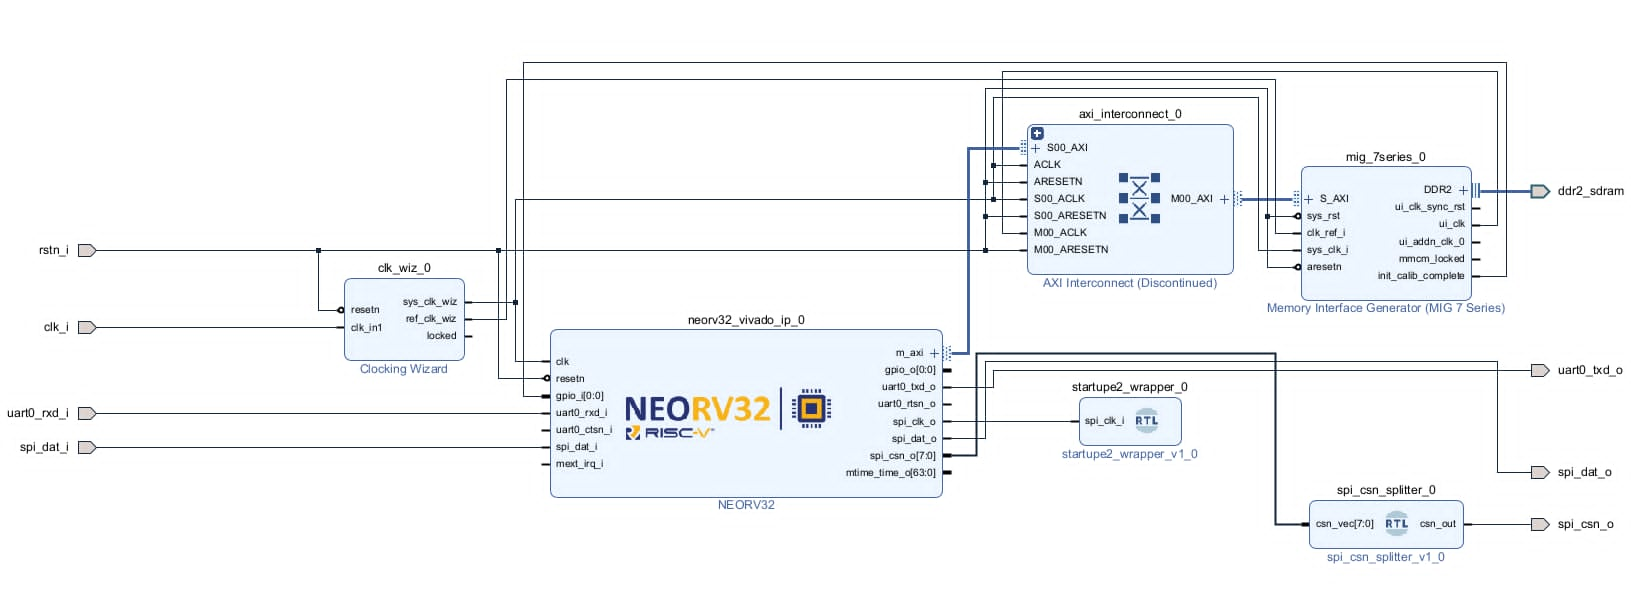
\includegraphics[width =1.2\textwidth]{Figures/blokk_diag.jpg}
    \caption{Block diagram of the full system, showing the NEORV32 processor 
    connected to DDR2 SDRAM via the AXI interconnect and MIG controller, and 
    to QSPI Flash via the SPI peripheral and STARTUPE2 wrapper. \textcolor{red}{MIDLERTIDIG, LAG I DRAW.IO}}
    \label{fig:sys_arch}
\end{figure}

The overall architecture is organized around three tiers of memory with distinct access characteristics. The trained model is stored persistently in on-board QSPI Flash, which survives power cycles but is too slow for direct inference use. At boot, the model is transferred from Flash into DDR2 SDRAM, which provides sufficient capacity for the full model and faster sequential access. During inference, model data is moved from DDR2 into the processor's internal DMEM, where clause evaluation is performed from fast on-chip storage.

The NEORV32 processor is connected to DDR2 through the XBUS interface, using a Wishbone-to-AXI4 bridge and a Xilinx MIG controller. QSPI Flash is accessed through the NEORV32 SPI peripheral. A Custom Functions Unit (CFU) is integrated directly into the CPU pipeline to accelerate clause evaluation using custom RISC-V instructions. Communication with a host PC is handled over UART at 921600 baud. The host sends booleanized input samples and receives predicted class labels together with cycle-accurate timing measurements.


% -------------------------------------
%   Hardware Platform Configuration
% -------------------------------------
\section{Hardware Platform Configuration}

\subsection{NEORV32 Instantiation on Nexys A7}

\subsection{DDR2 Integration and Memory Mapping}

\subsection{QSPI Flash Integration}

% -------------------------------------
%   TM Model Training and Serialization
% -------------------------------------
\section{Tsetlin Machine Model Training and Serialization}
\label{sec:model_rep}

\subsection{Training Configuration and Host-Side Execution}
\label{sec:training_config}

The TM model is trained on a host PC using the fast-tsetlin-machine repository \cite{cair_fast_tm_mnist}, a C implementation of the TM that uses bitwise operators for increased training and inference speed. The repository provides a binarized form of the MNIST dataset, with a threshold value of 0.3, meaning all pixel values above 0.3 are set to 1, and the remaining pixels are set to 0. The hyperparameters used during training are shown in Table \ref{tab:tm_hyperparams}.

\begin{table}[H]
\centering
\caption{Training hyperparameters for the MNIST TM model.}
\label{tab:tm_hyperparams}
\begin{tabular}{ll}
\hline
Parameter & Value \\ \hline
Clauses per class & 2000 \\
Threshold $T$ & 50 \\
Sensitivity $s$ & 10.0 \\
TA states & 8 \\
Epochs & 1 \\
Classes & 10 \\ \hline
\end{tabular}
\end{table}

As accuracy is not a priority in this project, only a single training epoch used to save time. The focus is instead on inference performance, meaning the only concern is that the different inference programs evaluated later are running the same model and achieve the same accuracy.

The TM training algorithm relies on stochastic feedback, which is implemented using floating-point arithmetic in the fast-tsetlin-machine repository. The NEORV32 does not include a floating-point unit, meaning all floating-point computations are very slow \cite{Nolting2024Datasheet}. Due to this it was decided that while entirely possible to implement, on-chip training would be outsite of the scope of this work as the possible performance gains introduced by custom instructions would be negligible compared to the overall training time.


\subsection{Action Bit Plane Extraction}
\label{sec:action_bit_plane}

During training of the TM, the full model is stored, including TA states, meaning 8 bits per literal. As mentioned in Section \ref{sec:tm_ta}, only the action bit (include or exclude) of each literal, or the action bit plane, is needed to perform inference. While discarding the state bits hinders on-chip learning, this reduces model size by a factor of the number of TA states, or in this case 8. 

Custom functions were added to the training repository to extract the action bit plane and serialize it to a binary a binary file \textcolor{red}{cite appendix}. For each class and each clause, the function writes 25 positive literal words followed by 25 negative literal words, each word being a 32-bit unsigned integer.

\subsection{Literal Layout and the Mixed-Word Problem}
\label{sec:literal_layout}

The internal \texttt{ta\_state} array in the fast-tsetlin-machine repository stores the action bit plane as a packed bitfield across \texttt{LA\_CHUNKS} 32-bit words per clause, with $\texttt{LA\_CHUNKS} = (\text{\#literals}\div 32)$ \cite{cair_fast_tm_mnist}. For MNIST with 784 features, the literal vector contains 1568 bits (784 positive and 784 negative literals), requiring 49 32-bit words to store all literal actions. Since $784 = 24 \times 32 + 16$, the positive and negative literal regions do not fall on a 32-bit word boundary. Word 25 contains the 16 remaining positive literal bits in its  lower half and the first 16 negative literal bits in its upper half. This mixed word makes it impossible to directly separate positive and negative literal masks on a per-word basis, which is required by the CFU instruction designs described in Section~\ref{sec:cfu_impl}.


To resolve this, a zero-padded layout was used when serializing the model. Each clause is stored as 25 positive literal words followed by 25 negative literal words, for a total of 50 words per clause. The boundary words (25 and 50) are split in half, with the lower 16 bits containing literals and the uper 16 bits zeroed. This is illustrated in Figure \ref{fig:mixed_word}.

\begin{figure}[H]
    \centering
    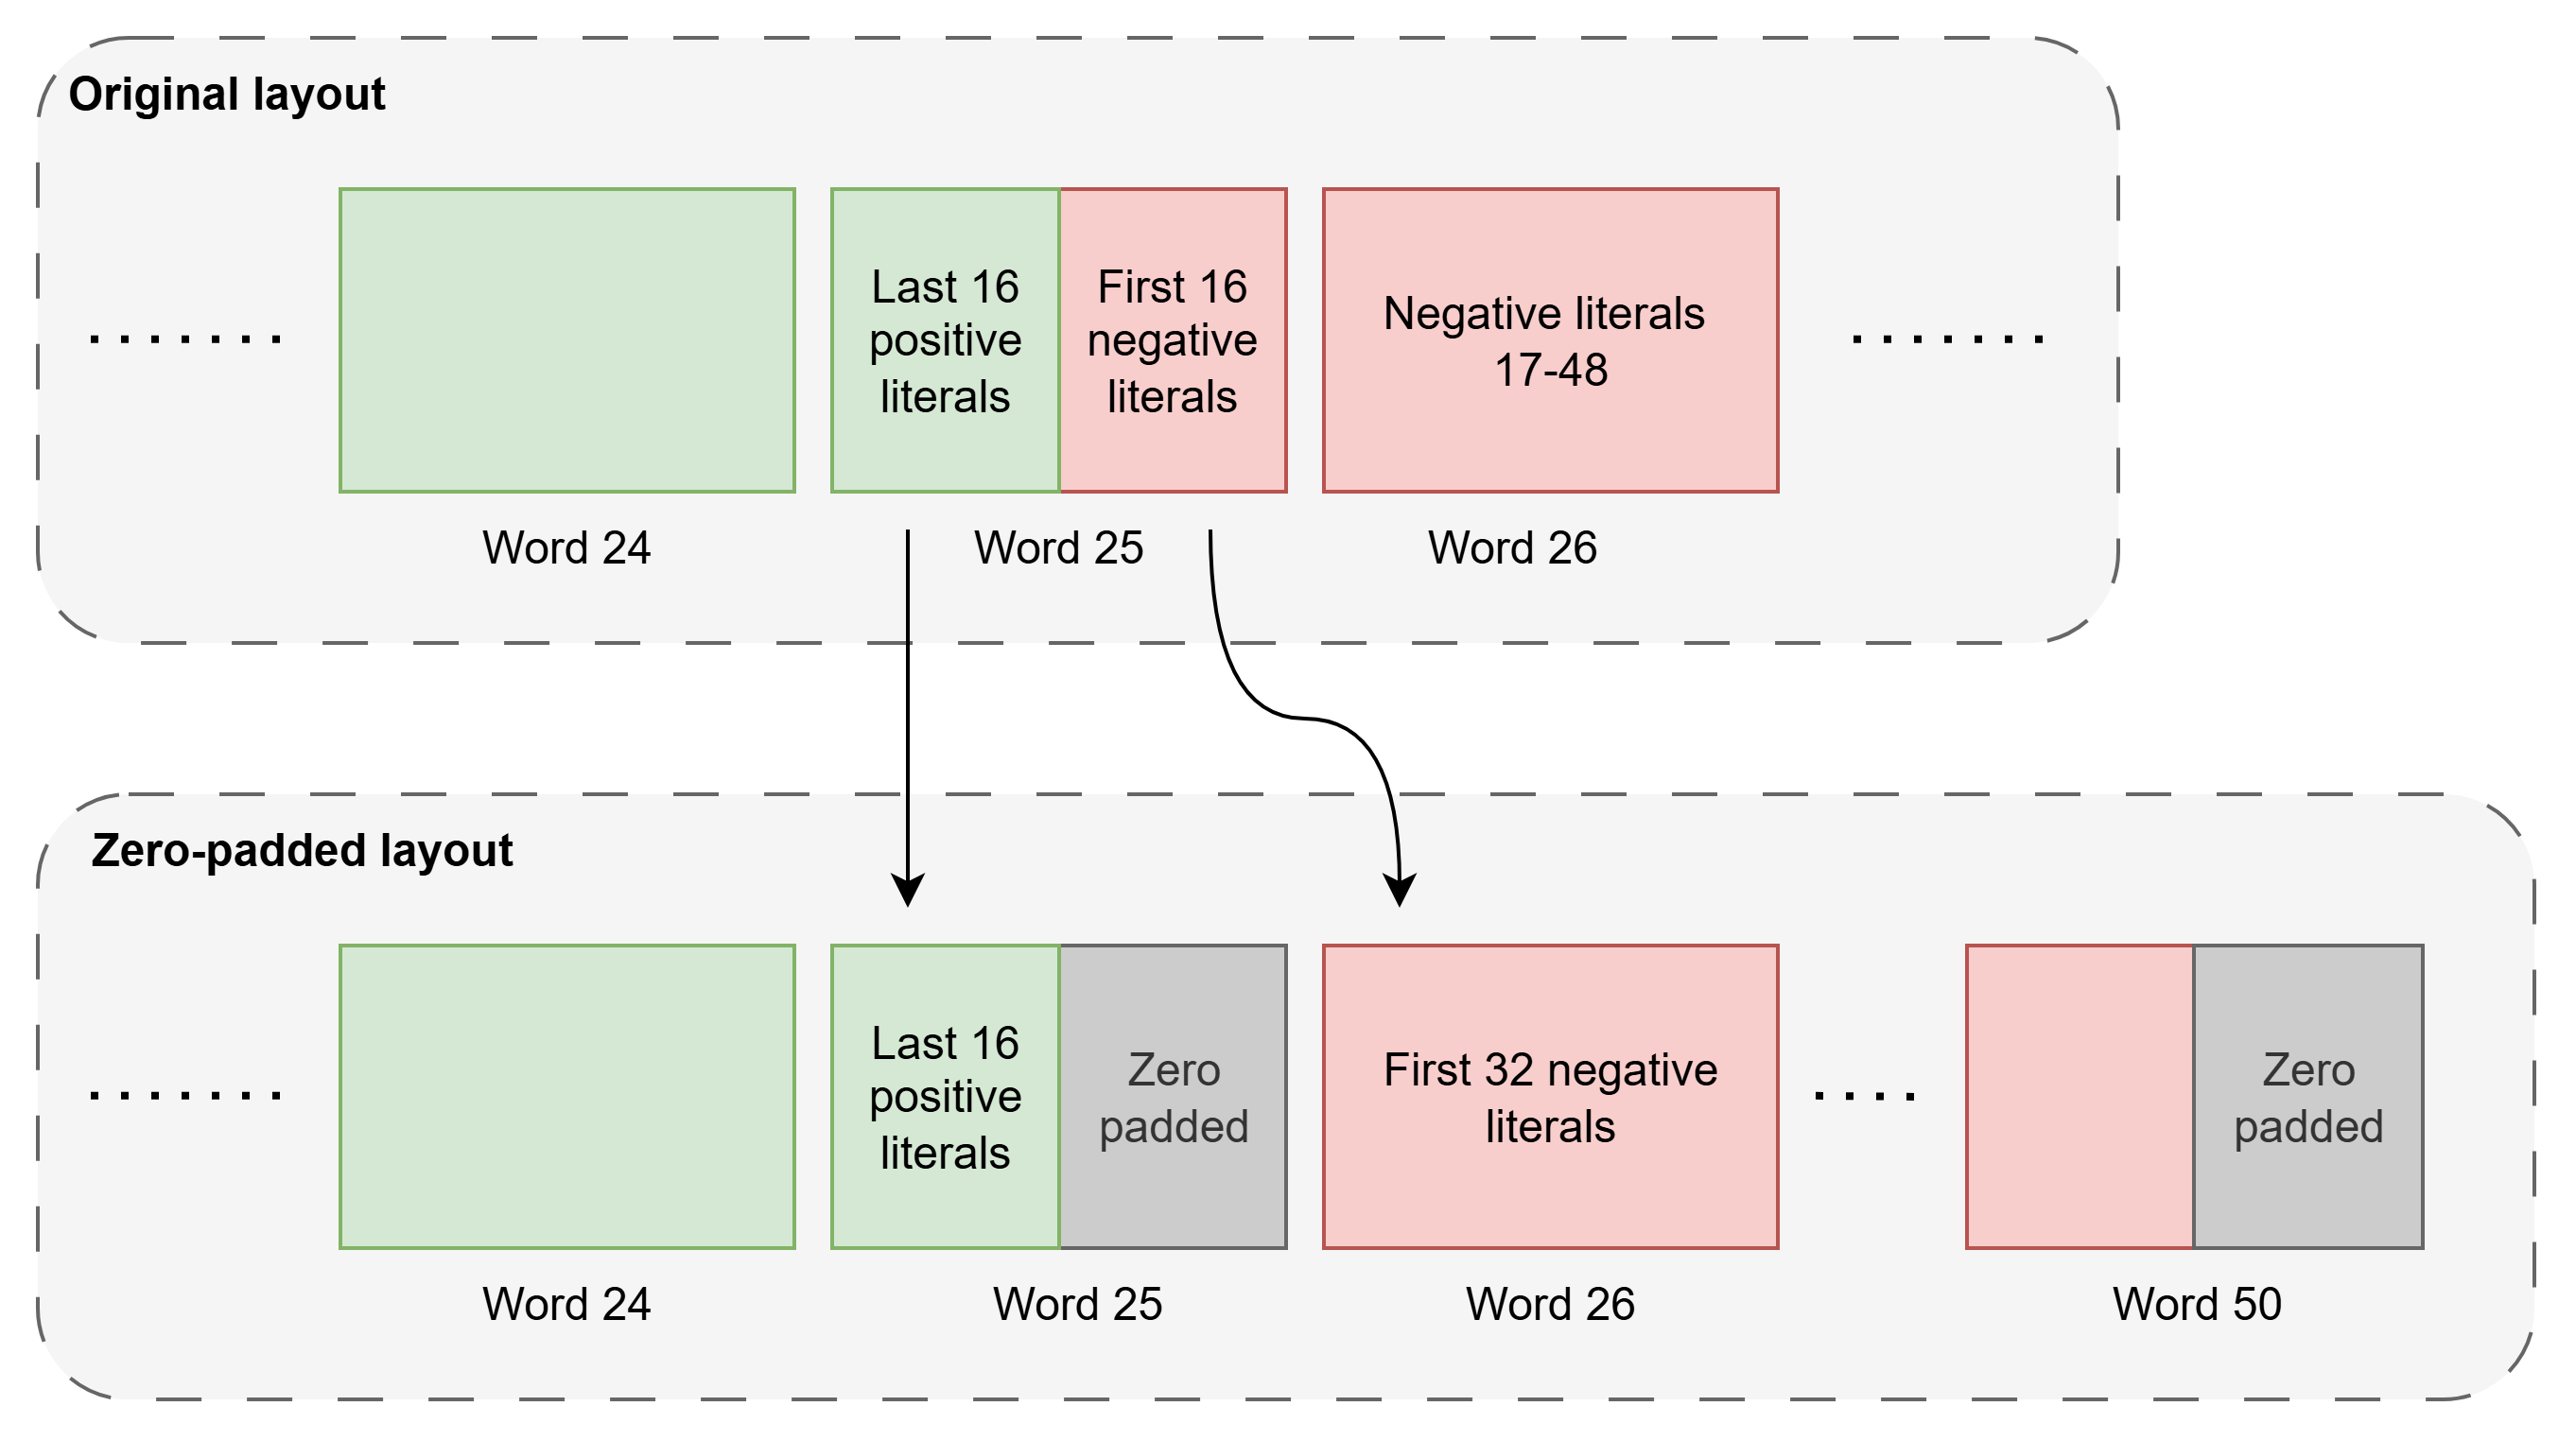
\includegraphics[width =1.0\textwidth]{Figures/mixed_word_problem.png}
    \caption{Comparison of the original 49-word literal layout and the 
    zero-padded 50-word layout. The zero-padded layout splits word 25 so that all words contain either only positive or only negative literals.}
    \label{fig:mixed_word}
\end{figure}

The resulting model sizes for the two layouts are summarized in
Table~\ref{tab:model_sizes}.

\begin{table}[H]
\centering
\caption{Model sizes for the original and zero-padded literal layouts.}
\label{tab:model_sizes}
\begin{tabular}{c|ccc}
Layout      & Words per clause & Total size (bytes) & Total size (MB) \\ \hline
Original    & 49               & 3 920 000 bytes    & $\approx3.74\text{ MB}$          \\
Zero-padded & 50               & 4 000 000 bytes    & $\approx3.81\text{ MB}$     
\end{tabular}
\end{table}

Both layouts exceed the capacity of the processor's internal memories by a large margin, necessitating the multi-tier storage architecture described in Section~\ref{sec:hw_config}.

% ---------------
%   Model Storage and Transfer
% ---------------
\section{Model Storage and Transfer}

\subsection{Flash Write Protocol}

\subsection{Flash-to-DDR2 Transfer at Boot}

% -------------------------------------
%   Inference Pipeline
% -------------------------------------
\section{Inference Pipeline}

\subsection{Input Encoding and Preprocessing}

\subsection{Per-Chunk Load Strategy}

\subsection{Per-Class Load Strategy}

\subsection{Output and Response Format}

% -------------------------------------
%   CFU Implementations
% -------------------------------------
\section{CFU Implementation}
\label{sec:cfu_impl}

This section describes the two CFU designs developed to accelerate clause
evaluation during inference. In the baseline software implementation, evaluating
a single chunk of a clause requires several instructions to perform the bitwise
masking and comparison. The purpose of the custom instructions is to encapsulate
this work into hardware, reducing instruction count and execution overhead.

Both of the different CFU design are implemented as one or more R4-type instructions using the \texttt{custom-1} opcode. As mentioned Section \ref{sec:neorv32_cfu}, the R4-type format swaps the \textit{funct7} field of the R-type format for an additional source register \textit{rs3}. The three 32-bit source registers are used the store the input word, the positive literal mask and the negative literal mask.

The major difference between the two developed designs is how much of the inference pipeline is moved from software into hardware. The first design offloads only the evaluation of a single chunk, leaving clause voting and class scoring in software. The second design moves the entire scoring pipeline into the CFU, maintaining internal state across instructions so that clause voting and class-score accumulation are performed in hardware.

Both designs operate solely on the operands supplied to them by the CPU and are therefore independent of how the model is stored or loaded. Either design functions correctly with the per-chunk load strategy or the per-class load strategy described in Section~\ref{sec:inference_pipeline}, as the load strategy only determines where the operand words are read from before being passed to the instruction. The benchmark programs used in this work happened to use the per-class strategy, but this choice is incidental to the CFU designs themselves.

The C code snippets shown in this section are abstracted to focus on the CFU instruction calls. References to the model data are shown as a generic \texttt{clause} pointer rather than the specific memory buffer used in the benchmark programs.

\subsection{CFU Design 1: Single-Chunk Processing}
\label{sec:cfu_design1}

The first design implements a single custom instruction that evaluates one 32-bit chunk of a clause. The
operands are defined as follows:

\begin{itemize}
    \item \textit{rs1}: the 32 input bits $X$ for this chunk
    \item \textit{rs2}: the positive mask (PM), where bit $i$ is set if positive
    literal $x_i$ is included in the clause
    \item \textit{rs3}: the negative mask (NM), where bit $i$ is set if negative
    literal $\lnot x_i$ is included in the clause
    \item \textit{rd}: the result, with bit 0 holding the chunk result and bit 1
    holding the all-zero status
\end{itemize}

\subsubsection{Instruction Encoding and Hardware Implementation}
\label{sec:cfu_design1_logic}

The instruction is implemented as a purely combinational circuit, as the
internal logic is simple and the goal is to minimize overhead. It evaluates the
clause-chunk condition shown in Equation~\eqref{eq:chunk_eval} by checking three
conditions in parallel:

\begin{equation}
\text{chunk ok} = \underbrace{((PM \land \lnot X) = 0)}_{\text{positive literals satisfied}}
\;\land\; \underbrace{((NM \land X) = 0)}_{\text{negative literals satisfied}}
\;\land\; \underbrace{((PM \lor NM) \neq 0)}_{\text{chunk not empty}}
\label{eq:chunk_eval}
\end{equation}

The three conditions are explained below:

\begin{enumerate}
    \item Positive literals satisfied: $(PM \land \lnot X) = 0$. If bit $i$ is
    set in PM, then $x_i$ must be 1 in the input. The expression
    $(PM \land \lnot X)$ identifies any included positive literals that are not
    satisfied. If the result is zero, all included positive literals are
    satisfied.

    \item Negative literals satisfied: $(NM \land X) = 0$. If bit $i$ is set in
    NM, then $x_i$ must be 0 in the input. The expression $(NM \land X)$
    identifies any included negative literals that are not satisfied. If the
    result is zero, all included negative literals are satisfied.

    \item Chunk not empty: $(PM \lor NM) \neq 0$. This indicates whether the
    chunk includes any literals at all. A chunk where both masks are zero
    contributes nothing to the clause, and the all-zero status is returned in
    bit 1 so the software can track the all-exclude condition across chunks.
\end{enumerate}

Although the instruction is purely combinational, the NEORV32 CFU introduces a
fixed execution latency. According to the NEORV32 documentation, CFU
instructions incur a minimum overhead of three clock cycles, independent of the
internal logic of the instruction \textcolor{red}{nrv32 datasheet cite}. The full VHDL
implementation is given in \textcolor{red}{fyll ut appendix og ref til det her}.

\subsubsection{Software Integration and Early-Exit Optimization}
\label{sec:cfu_design1_sw}

The instruction is accessed from C through the NEORV32 CFU intrinsic interface,
which translates the call into a single RISC-V instruction. For readability it
is wrapped in a macro, as shown in Listing~\ref{lst:cfu1_macro}.

\begin{code}
\captionof{listing}{Macro wrapping the Design 1 clause-chunk instruction.}
\label{lst:cfu1_macro}
\begin{minted}{c}
#define TM_CFU_CLAUSE_EVAL(x_bits, pos_mask, neg_mask) \
    neorv32_cfu_r4_instr(   \
        TM_FUNCT3_CLAUSE,   \
        (uint32_t)(x_bits), \
        (uint32_t)(pos_mask), \
        (uint32_t)(neg_mask)  \
    )
\end{minted}
\end{code}

For each clause, the software iterates over the 25 chunks, calling the instruction for each non-empty chunk and breaking out of the loop as soon as a chunk fails. The clause output, the all-exclude check, the clause vote, and the class-score accumulation are all handled in software, in the same way as the baseline version. The integration is shown in Listing~\ref{lst:cfu1_c}.

\begin{code}
\captionof{listing}{Software integration of CFU Design 1. The clause vote and 
class scoring are performed in software.}
\label{lst:cfu1_c}
\begin{minted}{c}
for (int j = 0; j < CLAUSES; j++) {
    for (int k = 0; k < POS_CHUNKS; k++) {
        uint32_t pos = clause[k];
        uint32_t neg = clause[POS_CHUNKS + k];

        if ((pos | neg) == 0) continue;
        all_exclude = 0;
        
        // Bitwise checks on positive and negative 
        // literals  is handled in hardware
        uint32_t chunk_ok = TM_CFU_CLAUSE_EVAL(Xi[k], pos, neg);

        if (!chunk_ok) { clause_out = 0; break; }
    }

    clause_out = clause_out && !all_exclude;
    // Score accumulation based on clause polarity
    // (even clauses vote for the class, odd vote against)
    if (clause_out) {
        if ((j & 1) == 0) class_sum++;
        else              class_sum--;
    }
}

\end{minted}
\end{code}

The early exit on the first failing chunk avoids issuing further instructions for a clause that has already failed, mirroring the early-exit optimization used in the baseline software implementation.

\subsection{CFU Design 2: Stateful Clause Processing}
\label{sec:cfu_design2}

The second design moves the full scoring pipeline into the CFU. Rather than returning a per-chunk result for the software to combine, this design maintains internal state across instructions, accumulating clause outcomes into a running class score entirely in hardware. It is implemented as a sequential circuit, with state held in registers between instruction calls.

\subsubsection{Instruction Set and State Management}
\label{sec:cfu_design2_logic}

The design holds three internal state signals: a flag indicating whether the current clause has failed (\texttt{clause\_failed}), a flag indicating whether the current clause has so far included no literals (\texttt{clause\_all\_exclude}), and the accumulated class score (\texttt{class\_score}). Three custom operations, selected by the \texttt{funct3} field, manipulate this state as shown in Figure \ref{fig:cfu_fsm}.

\begin{figure}[H]
    \centering
    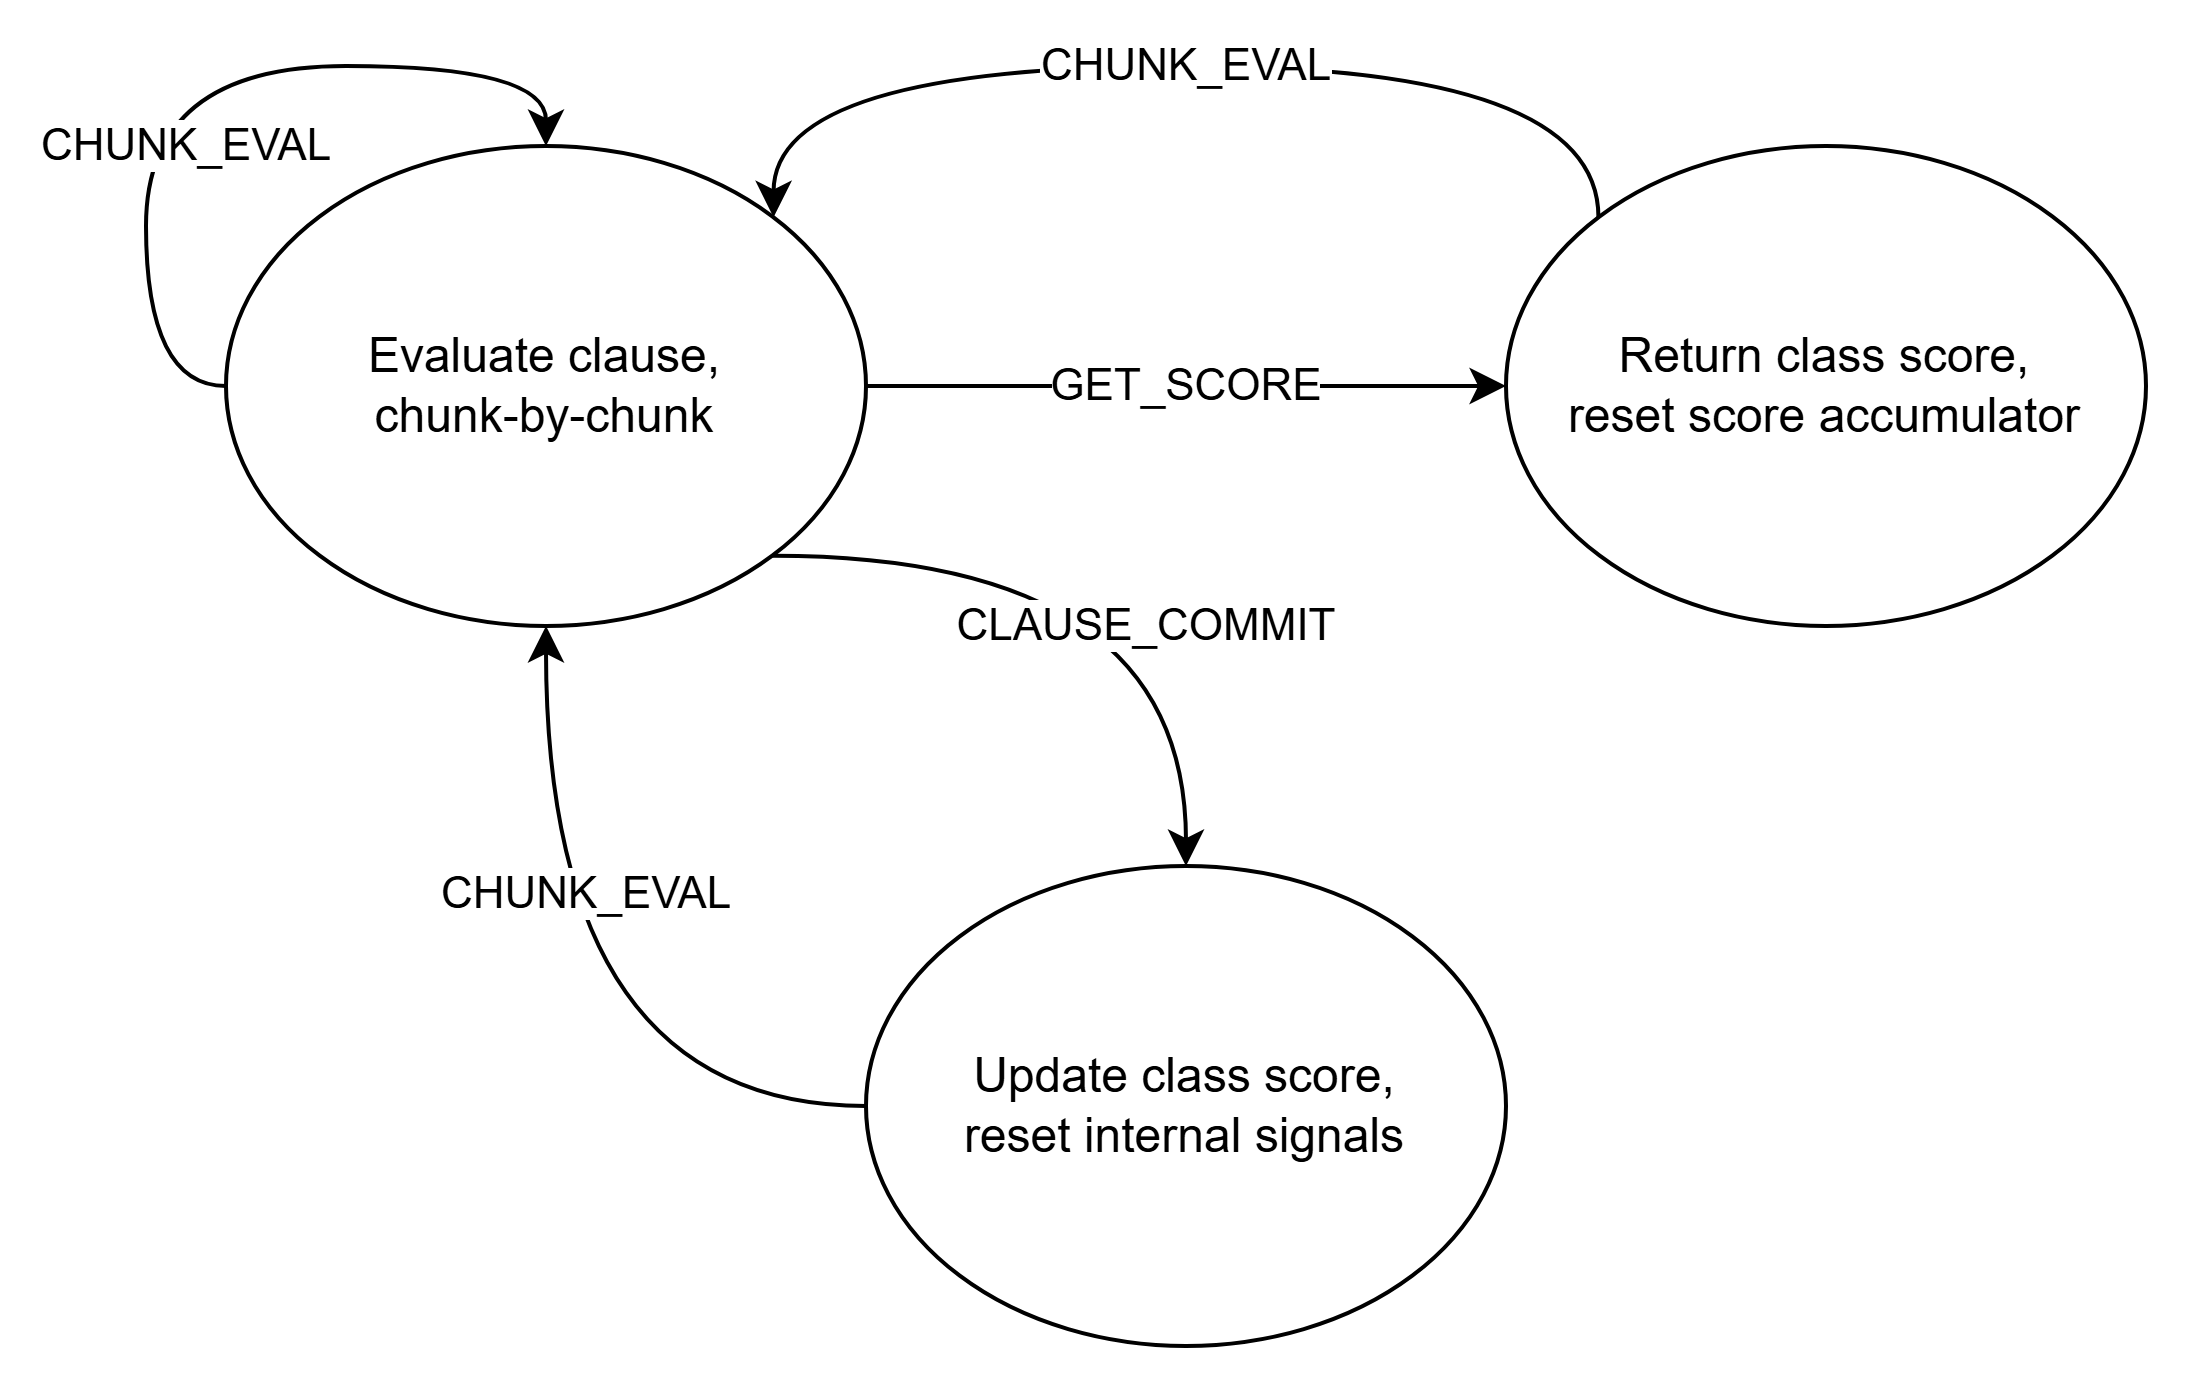
\includegraphics[width=0.9\textwidth]{Figures/cfu2_states.png}
    \caption{State diagram of the second CFU design.}
    \label{fig:cfu_fsm}
\end{figure}

The different instructions implemented in the second design operate as follows:

\begin{itemize}
    \item \texttt{CHUNK\_EVAL} evaluates one chunk using the same mismatch and all-zero logic as in the first design, and updates the clause-failed and all-exclude state accordingly. It returns the current clause-failed status, allowing the software to break out of the chunk loop early once a clause has failed.
    \item \texttt{CLAUSE\_COMMIT} finalizes the current clause. If the clause did not fail and was not all-exclude, it adds the clause vote to the class score, with the vote determined by wether the clause votes for or against the current class, based on the clause id. The clause-failed and all-exclude flags are then reset for the next clause. The class score is clamped to the threshold $T$ during accumulation.
    \item \texttt{GET\_SCORE} returns the final clamped class score as a signed 32-bit value and resets the score accumulator for the next class.
\end{itemize}

By performing the vote accumulation and threshold clamping in hardware, this design removes the per-clause and per-class scoring arithmetic from the software loop entirely. Like in the first design, each operation incurs the fixed three cycle CFU latency, as all operations complete in a single cycle.

\subsubsection{Software Integration}
\label{sec:cfu_design2_sw}

Like in the first CFU design, the different instructions are invoked through C macros, as shown in Listing \ref{lst:cfu2_macros}

\begin{code}
\captionof{listing}{Macros wrapping the three different Design 2 instructions.}
\label{lst:cfu2_macros}
\begin{minted}{c}
#define TM_FUNCT3_CLAUSE_COMMIT 0b001
#define TM_FUNCT3_CHUNK_EVAL    0b000
#define TM_FUNCT3_GET_SCORE     0b010

#define CFU_CHUNK_EVAL(x_bits, pos_mask, neg_mask) \
    neorv32_cfu_r4_instr(          \
        TM_FUNCT3_CHUNK_EVAL,      \
        (uint32_t)(x_bits),        \
        (uint32_t)(pos_mask),      \
        (uint32_t)(neg_mask)       \
    )
#define CFU_CLAUSE_COMMIT(clause_idx) \
    neorv32_cfu_r4_instr(            \
        TM_FUNCT3_CLAUSE_COMMIT,     \
        (uint32_t)(clause_idx),      \
        0,                           \
        0                            \
    )
#define CFU_GET_SCORE() \
    (int32_t)neorv32_cfu_r4_instr( \
        TM_FUNCT3_GET_SCORE,        \
        0,                          \
        0,                          \
        0                           \
    )
\end{minted}
\end{code}


In software, the inner chunk loop calls \texttt{CHUNK\_EVAL} for each non-empty chunk, breaking early if the clause has failed. After the chunk loop, a single \texttt{CLAUSE\_COMMIT} call finalizes the clause. Once all clauses of a class have been processed, a single \texttt{GET\_SCORE} call retrieves the class score. The software no longer tracks clause outputs or accumulates votes, as shown in Listing~\ref{lst:cfu2_c}.

\begin{code}
\captionof{listing}{Software integration of CFU Design 2. Clause voting and class scoring are performed entirely in the CFU.}
\label{lst:cfu2_c}
\begin{minted}{c}
for (int j = 0; j < CLAUSES; j++) {
    const uint32_t *clause = &model[j * WORDS_PER_CLAUSE];

    for (int k = 0; k < POS_CHUNKS; k++) {
        if ((clause[k] | clause[POS_CHUNKS + k]) == 0) continue;

        if (CFU_CHUNK_EVAL(Xi[k], clause[k], clause[POS_CHUNKS + k]) & 1) {
            break;
        }
    }

    CFU_CLAUSE_COMMIT(j);
}

int class_sum = (int)CFU_GET_SCORE();
\end{minted}
\end{code}

\subsection{Design Comparison}
\label{sec:cfu_comparison}

The two designs represent different points on the spectrum of hardware versus
software partitioning of the inference pipeline. Design 1 offloads only the
innermost operation, the evaluation of a single chunk, and leaves all clause
voting and class scoring in software. This keeps the hardware minimal and the
instruction purely combinational. Design 2 offloads the entire scoring pipeline,
performing clause voting, class-score accumulation, and threshold clamping in
hardware, at the cost of a more complex sequential design that must maintain
internal state and that requires additional commit and score-retrieval
instructions per clause and per class.

The motivation for Design 2 was to investigate whether moving a larger portion
of the inference pipeline into hardware would yield a further performance
improvement over Design 1. The performance of both designs relative to the
baseline software implementation is reported and analysed in the next chapter.






\chapter{Results}
% -------------------------------------
%   Benchmark Methodology
% -------------------------------------


% -------------------------------------
%   Memory Architecture Evaluation
% -------------------------------------


% -------------------------------------
%   CFU Performance Evaluation
% -------------------------------------


% -------------------------------------
%   Resource Utilization
% -------------------------------------



\chapter{Discussion}
\label{chap:discussion}
% -------------------------------------
%   Bottleneck Analysis
% -------------------------------------
\section{Bottleneck Analysis}

% -------------------------------------
%   CFU Effectiveness and Latency Trade-Offs
% -------------------------------------
\section{CFU Effectiveness and Latency Trade-Offs}

% -------------------------------------
%   Model Format Design Decisions
% -------------------------------------
\section{Model Format Design Decisions}

% -------------------------------------
%   Limitations
% -------------------------------------
\section{Limitations}

% -------------------------------------
%   Comparison with Related Works
% -------------------------------------
\section{Comparison with Related Works}

% -------------------------------------
%   Future Work
% -------------------------------------
\section{Future Work}

\subsection{CFS + DMA architecture}

\subsection{DDR2 burst transfers}

\subsection{Nonempty chunk bitmask} % spør claude hva dette i det hele tatt betyr lmao

\subsection{On-chip training feasibility}




\chapter{Conclusions}
This thesis set out to explore whether or not the clause evaluation speedup achieved on the small NoisyXOR problem in a preceding project thesis \textcolor{red}{cite jonas den kule} carries over to MNIST scale, where the TM model far exceeds the on-chip memory of the NEORV32 processor and must reside in external memory (DDR2 SDRAM) at run time. To answer this, a multi-class MNIST TM with 2000 clauses per class was deployed on a Nexys A7 board featuring a Xilinx Artix-7 FPGA, and three inference implementations, a baseline software version and two CFU designs, were evaluated under a per-chunk and a per-class model load strategy.

The measurements lead to a clear conclusion. All six configurations achieved similar classification accuracy, confirming that every implementation evaluates the same model. The custom instructions, however, produced no meaningful speedup, with the simpler combinatorial CFU design improved inference speed by less than 1\%, and the more complex stateful CFU design performing worse than the baseline implementation. This stands in sharp contrast to the $4.42\times$ speedup reported at NoisyXOR scale.

The reason for this is a shift in the where the bottleneck of inference lies. At MNIST scale, moving the model out of DDR2, rather than evaluating clauses, takes up a majority of inference time.  In the per-class strategy the model preload alone accounts for approximately 91\% of the total, and the effective transfer rate of around 5.1\,MB/s reaches only a fraction of the maximum bandwidth the DDR2 device, indicating that the per-transaction overhead on single-word reads, not the memory device itself, is the limiting factor. Clause scoring contributes too small a share of inference time for any clause-level instruction to influence the result. The bottleneck is therefore not fixed by the algorithm but moves with the scale of the model, and at a realistic problem size it is the memory hierarchy rather than the computational power that limits performance.

These findings reframe processor-level TM acceleration as a memory problem rather than a compute problem once the model no longer fits on-chip. This opens up new directions for future work to take, like accelerating transfer rate through DDR2 burst transfers, a hybrid load strategy that preserves early exit, or a wider processor-external accelerator. 

It is also worth looking at other TM variants such as the Coalesced and Convolutional TM, which achieve better accuracy with far fewer clauses, in turn making the models far smaller, in addition to them having heavier computation costs per-clause. These factors might shift the bottleneck away from memory accessing, and custom instructions might still be effective for acceleration. On-chip training is feasible, but likely only as a reduced-scale proof of concept. The custom instructions themselves were shown to be cheap and correct; the limiting factor lies not in their design but in where the performance cost of inference at scale actually resides.



\chapter*{AI Declaration}
\section*{Description of Use of Artificial Intelligence}

In working on this assignment, I have used artificial intelligence (AI) tools in the following ways: I used ChatGPT to assist with idea development and structuring of the text. AI was used to suggest phrasing and provide language improvements, but all content has been reviewed, edited, and academically assessed by me. AI was not used to generate entire paragraphs or to answer the assignment in its entirety. I have also not uploaded personal data or sensitive information into the AI tool. I am solely responsible for the academic content of the assignment.

\addcontentsline{toc}{chapter}{\protect\numberline{}References}
\printbibliography[title={References}] %you may change the title in the toc here if you want



\chapter*{\LARGE \textbf{Appendices}}
\fancyhf{} %clear the header, it should be empty for the appendices
\renewcommand{\headrulewidth}{0pt} %no rule
\fancyfoot[C]{\thepage} %set the page numbers in the center of the footer instead 

%it is possible to set a different page numbering style for the appendix, but I personally just continued with the same page numbering as the main content as I find that more tidy
%\pagenumbering{roman}
%\setcounter{page}{1}
\addcontentsline{toc}{chapter}{\protect\numberline{}Appendices:}
\appendix


\chapter{Github Repository}
% \addcontentsline{toc}{chapter}{\protect\numberline{}A - Github repository} 

All code used in this document are included in the Github repository linked below.
 
\url{https://github.com/joblob7488/master_code.git}


\chapter{CFU Design 1 VHDL}
\label{app:cfu1vhdl}
% \addcontentsline{toc}{chapter}{\protect\numberline{}B - CFU Design 1 VHDL} 
\inputminted[
    frame=lines,
    linenos,
    breaklines,
    breakanywhere,
    fontsize=\small
]{vhdl}{Code/neorv32_cpu_cp_cfu_combinatorial.vhd}


\chapter{CFU Design 2 VHDL }
\label{app:cfu2vhdl}
% \addcontentsline{toc}{chapter}{\protect\numberline{}C - CFU Design 2 VHDL } 
\inputminted[
    frame=lines,
    linenos,
    breaklines,
    breakanywhere,
    fontsize=\small
]{vhdl}{Code/neorv32_cpu_cp_cfu_sequential.vhd}


\chapter{Non-CFU Per-Chunk Inference}
% \addcontentsline{toc}{chapter}{\protect\numberline{}D - Non-CFU Per-Chunk Inference} 
\inputminted[
    frame=lines,
    linenos,
    breaklines,
    breakanywhere,
    fontsize=\small
]{c}{Code/tm_chunkload_noncfu.c}


\chapter{CFU Design 1 Per-Chunk Inference}
% \addcontentsline{toc}{chapter}{\protect\numberline{}E - CFU Design 1 Per-Chunk Inference} 
\inputminted[
    frame=lines,
    linenos,
    breaklines,
    breakanywhere,
    fontsize=\small
]{c}{Code/tm_chunkload_cfu1.c}


\chapter{CFU Design 2 Per-Chunk Inference}
% \addcontentsline{toc}{chapter}{\protect\numberline{}F - CFU Design 2 Per-Chunk Inference} 
\inputminted[
    frame=lines,
    linenos,
    breaklines,
    breakanywhere,
    fontsize=\small
]{c}{Code/tm_chunkload_cfu2.c}


\chapter{Non-CFU Per-Class Inference}
% \addcontentsline{toc}{chapter}{\protect\numberline{}G - Non-CFU Per-Class Inference} 
\inputminted[
    frame=lines,
    linenos,
    breaklines,
    breakanywhere,
    fontsize=\small
]{c}{Code/tm_preloadclass_noncfu.c}


\chapter{CFU Design 1 Per-Class Inference}
% \addcontentsline{toc}{chapter}{\protect\numberline{}H - CFU Design 1 Per-Class Inference} 
\inputminted[
    frame=lines,
    linenos,
    breaklines,
    breakanywhere,
    fontsize=\small
]{c}{Code/tm_preloadclass_cfu.c}


\chapter{CFU Design 2 Per-Class Inference}
% \addcontentsline{toc}{chapter}{\protect\numberline{}I - CFU Design 2 Per-Class Inference}
\inputminted[
    frame=lines,
    linenos,
    breaklines,
    breakanywhere,
    fontsize=\small
]{c}{Code/tm_preloadclass_cfu2.c}


\chapter{Benchmark Inference Python Script}
% \addcontentsline{toc}{chapter}{\protect\numberline{}J - Benchmark Inference Python Script}
\inputminted[
    frame=lines,
    linenos,
    breaklines,
    breakanywhere,
    fontsize=\small
]{python3}{Code/tm_benchmark.py}


\chapter{Python Model Transfer Script}
% \addcontentsline{toc}{chapter}{\protect\numberline{}K - Python Model Transfer Script}
\inputminted[
    frame=lines,
    linenos,
    breaklines,
    breakanywhere,
    fontsize=\small
]{python3}{Code/model_transfer.py}


\chapter{Write Model To Flash Script}
% \addcontentsline{toc}{chapter}{\protect\numberline{}L - Write Model To Flash Script}
\inputminted[
    frame=lines,
    linenos,
    breaklines,
    breakanywhere,
    fontsize=\small
]{c}{Code/write_model_to_flash.c}


\chapter{Python Exe Uploader Script}
\label{app:exe_uploader}
% \addcontentsline{toc}{chapter}{\protect\numberline{}M - Python Exe Uploader Script}
\inputminted[
    frame=lines,
    linenos,
    breaklines,
    breakanywhere,
    fontsize=\small
]{python3}{Code/uart_upload.py}


\end{document}
